% RMSD plot, Bar plot
% Tree graph colored by order, native contact, hydrogen bond
% structure figure
% Projection on free energy landscape

\begin{figure}[ht]
\begin{minipage}[b]{0.49\textwidth}
\centering
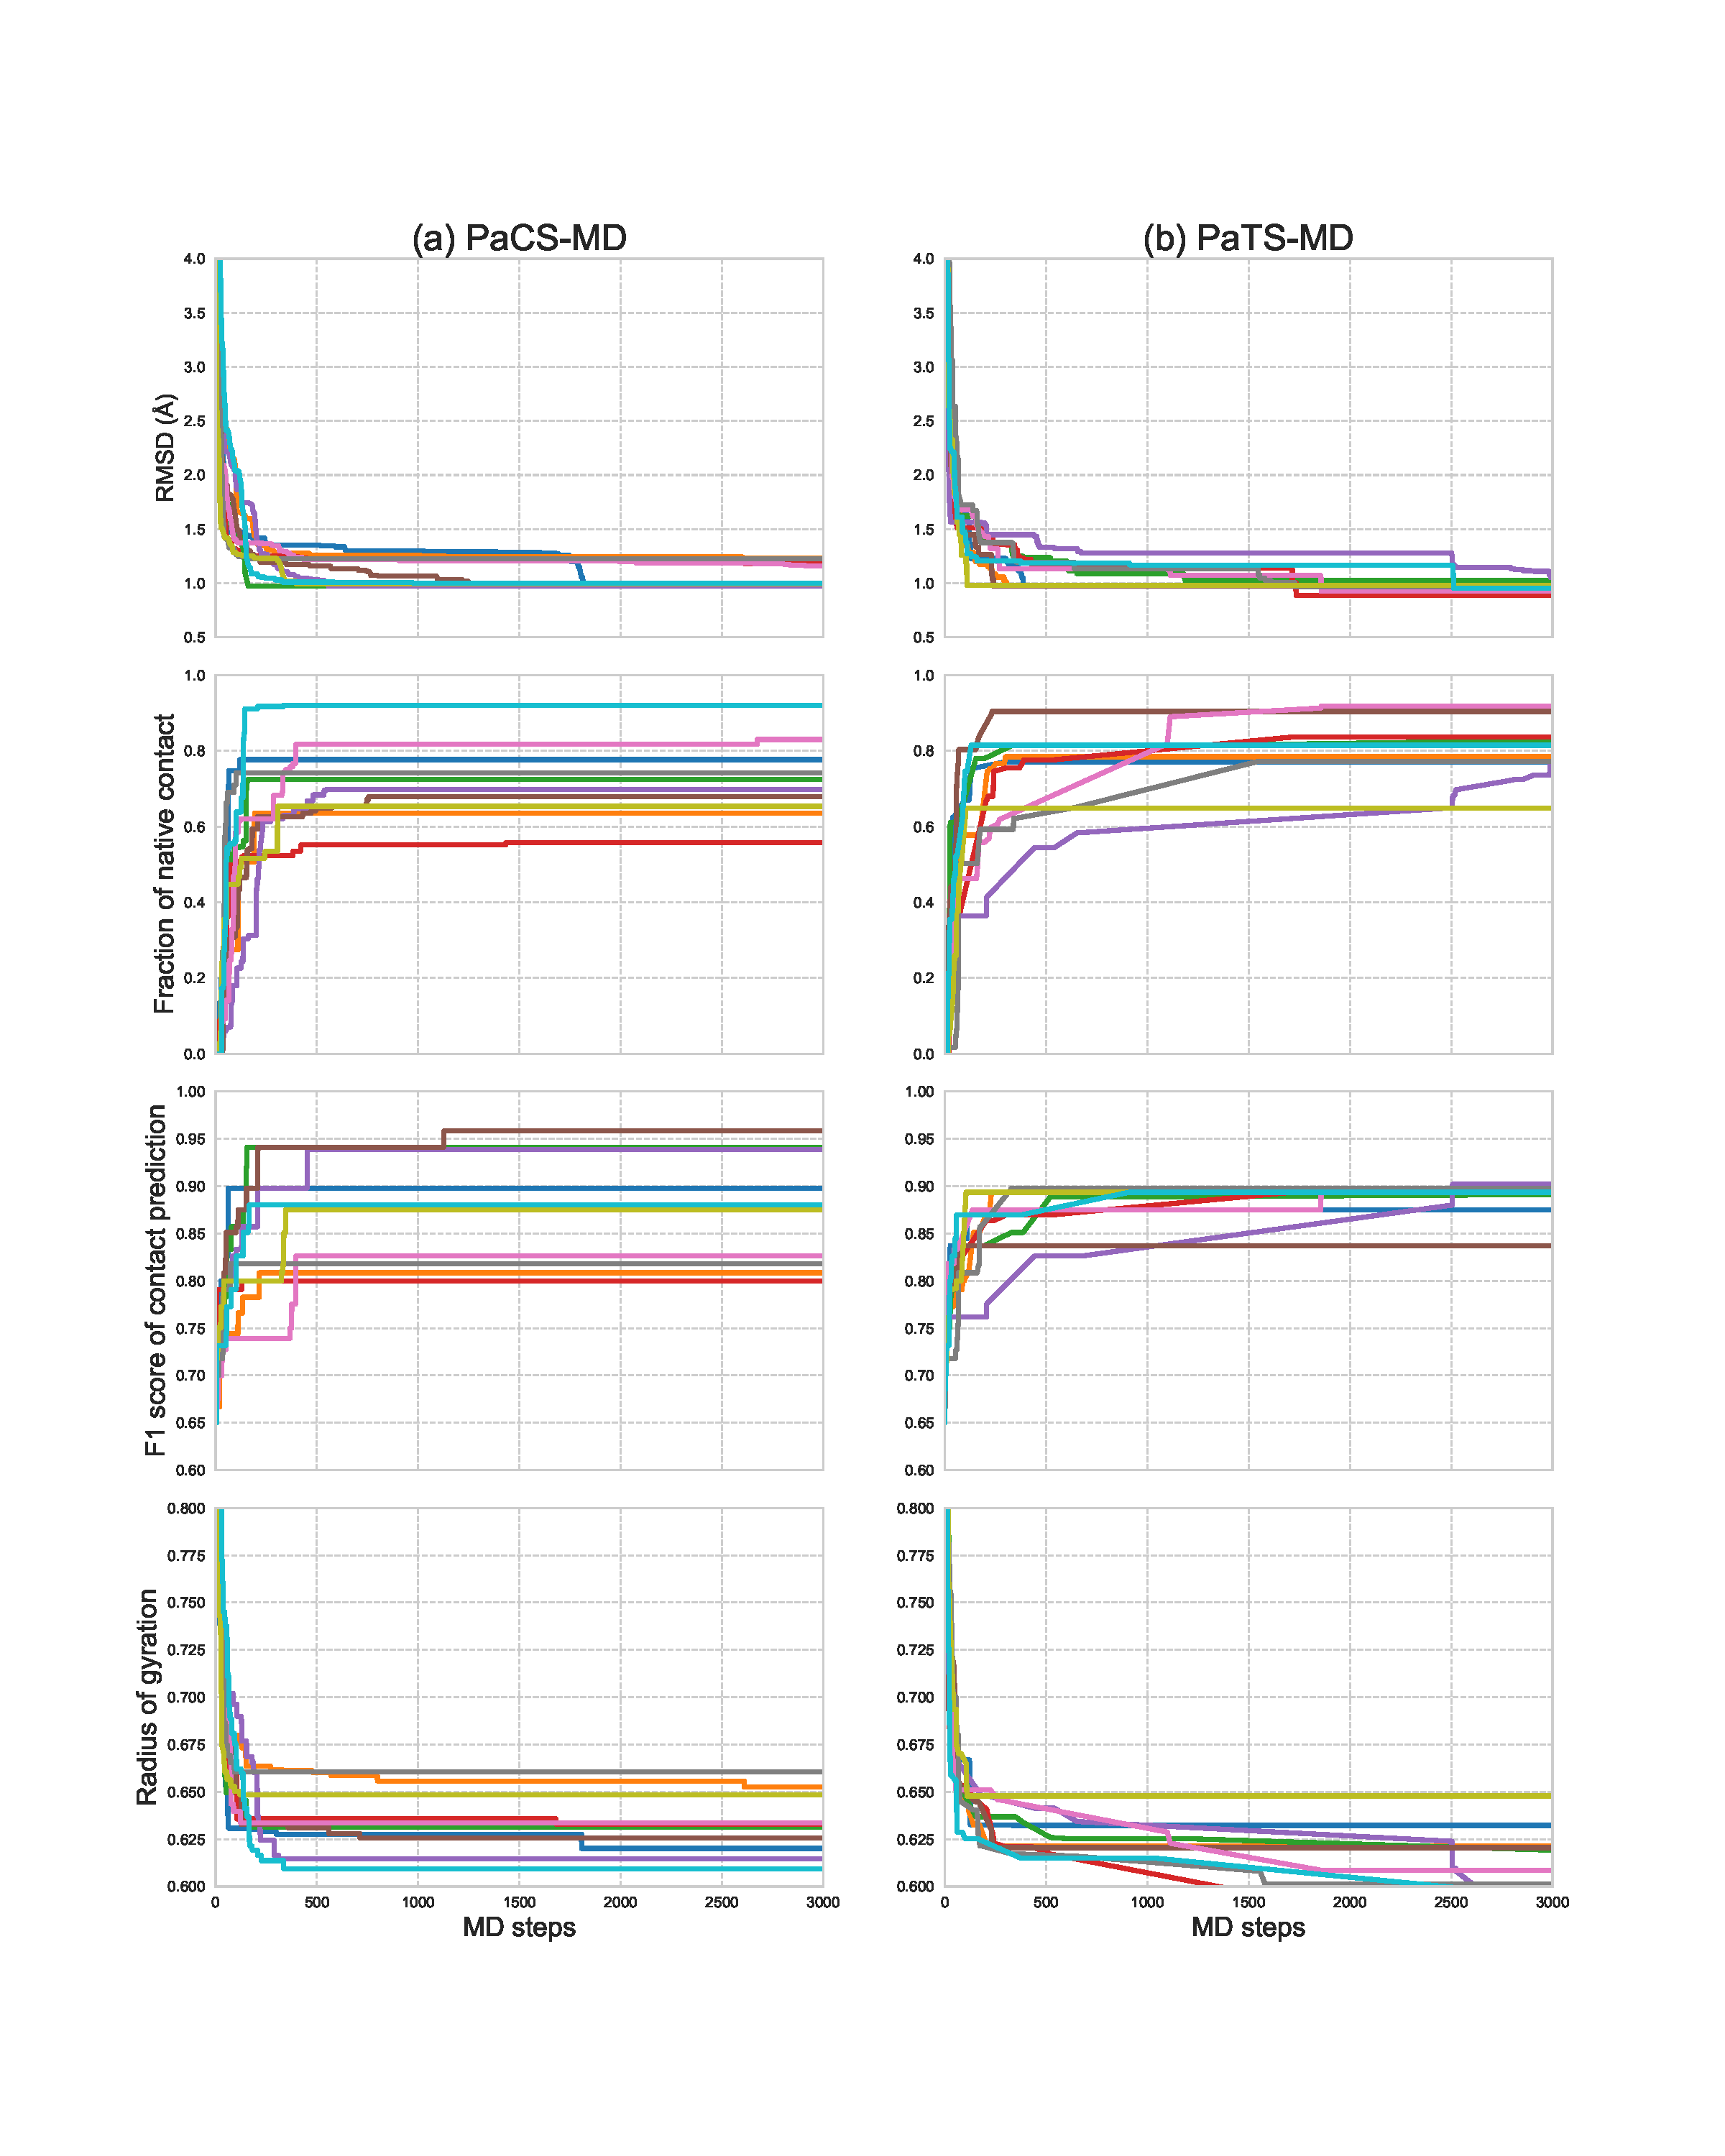
\includegraphics[width=1.0\textwidth]{Figures/chig_plot_both.pdf}
\caption{PaCS}
\label{fig:result_pacs_plot}
\end{minipage}
\begin{minipage}[b]{0.49\textwidth}
\centering
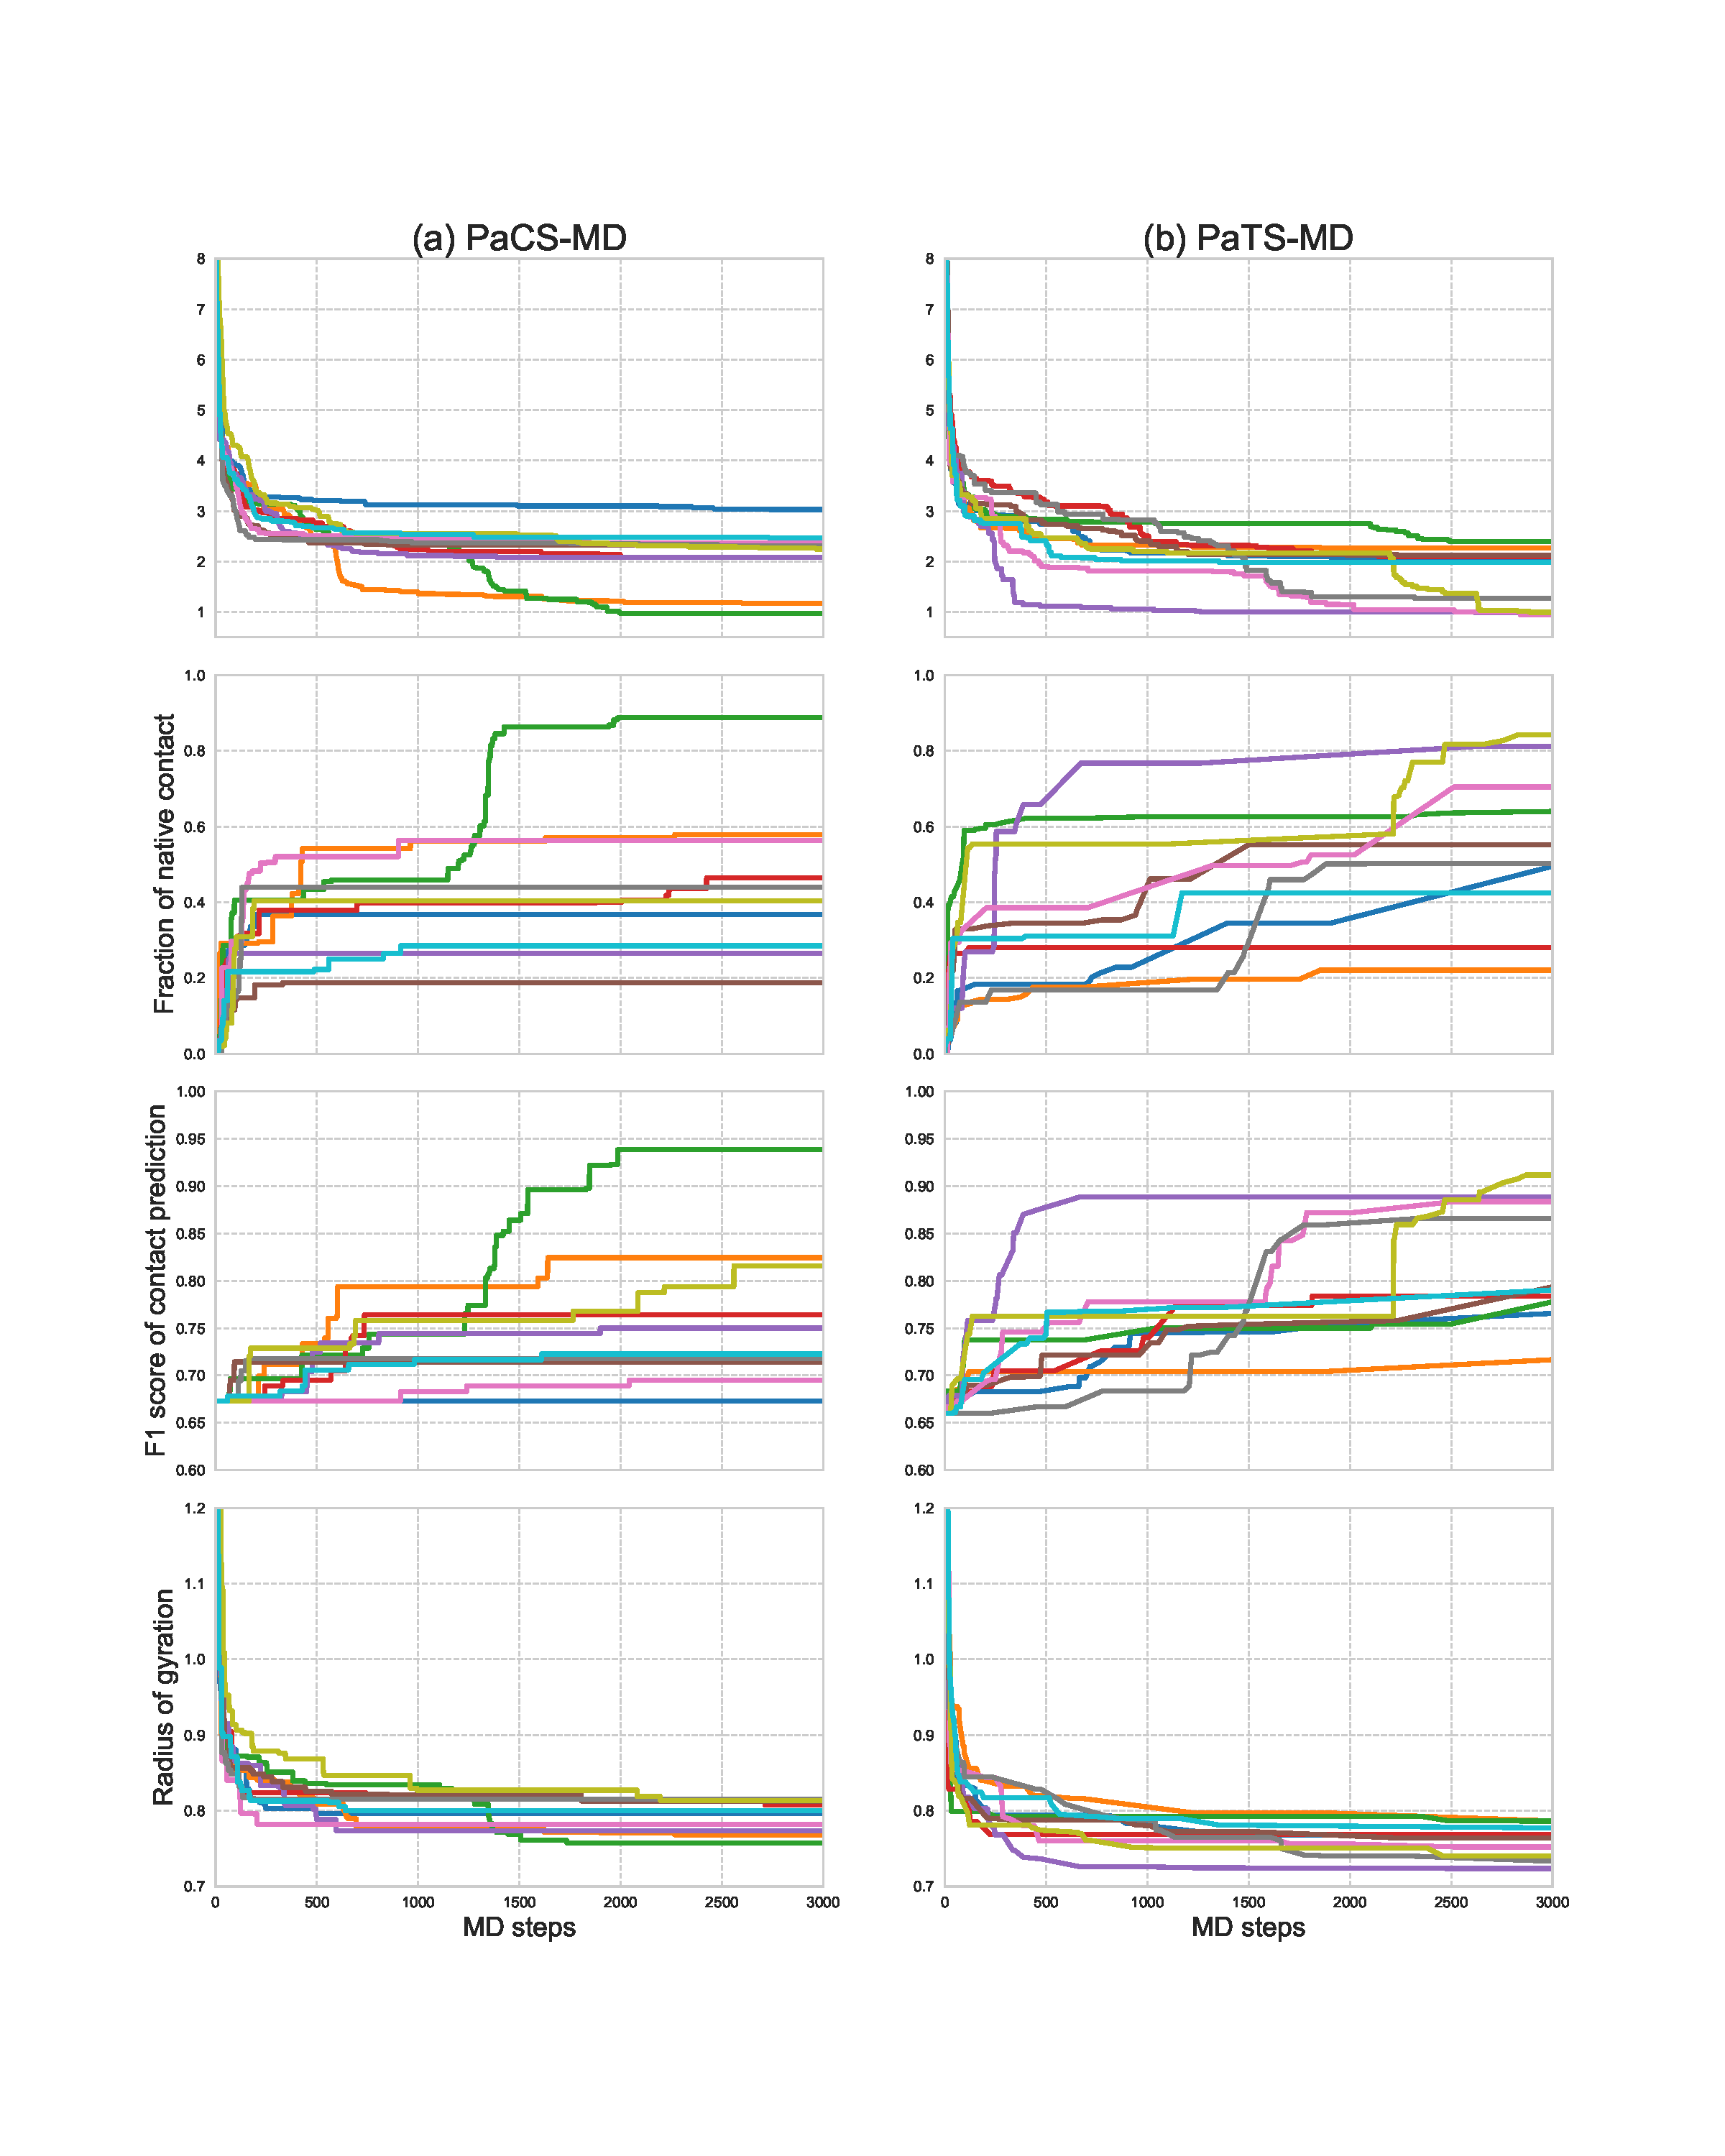
\includegraphics[width=1.0\textwidth]{Figures/trp_plot_both.pdf}
\caption{PaTS}
\label{fig:result_pats_plot}
\end{minipage}
\end{figure}

\begin{figure}[ht]
\begin{minipage}[b]{0.95\textwidth}
\centering
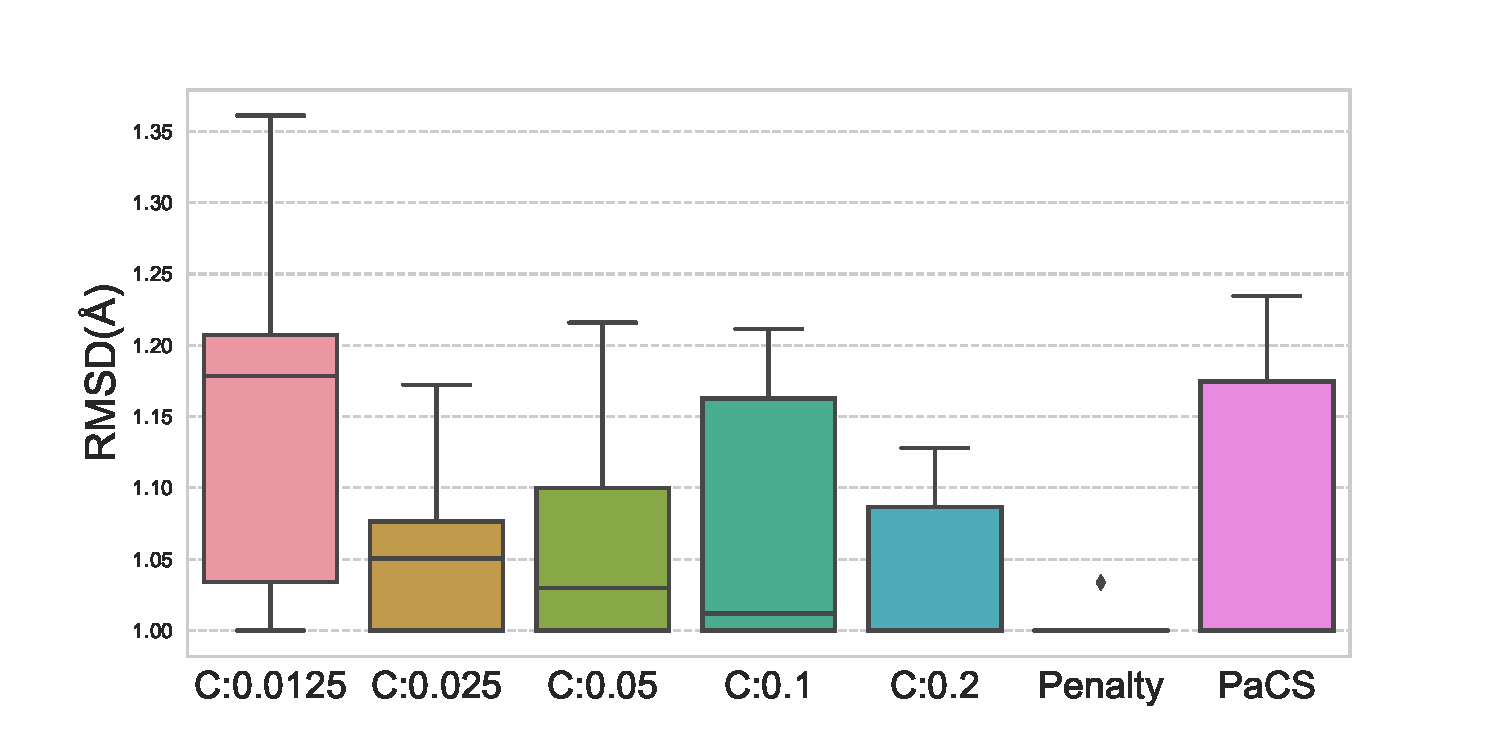
\includegraphics[width=0.9\textwidth]{Figures/chignolin_result_boxplot.pdf}
\subcaption{Chignolin}
\end{minipage}
\begin{minipage}[b]{0.95\textwidth}
\centering
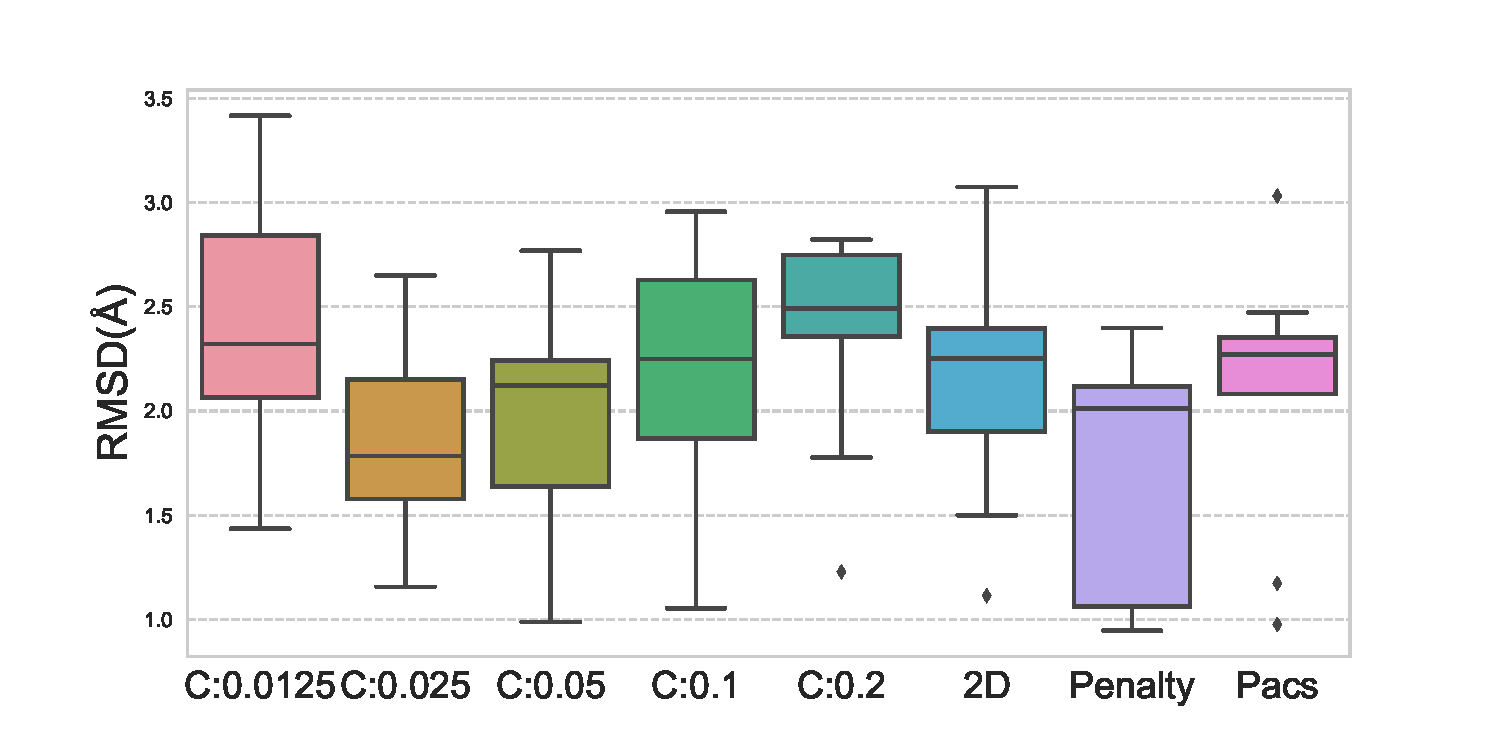
\includegraphics[width=0.9\textwidth]{Figures/trpcage_result_boxplot.pdf}
\subcaption{Trp-cage}
\end{minipage}
\caption{Boxplot}
\label{fig:result_box}
\end{figure}


\subsection{Chignolin Folding}
To search the reactive trajectories of folding pathway of Chignolin in explicit solvent, PaCS-MD and PaTS-MD were performed up to 3000 MD steps. In PaTS-MD, $C$ was set to 0.05 and penalization parameter $\alpha$ was set to 1.05. 

Figure \ref{fig:result_pacs_plot} shows various profiles of 10 trials of PaCS-MD and PaTS-MD as a function of MD steps, which includes RMSD, fraction of native contact, f1 score of contact prediction and radius of gyration. (An explanation of fraction and f1). 
This profiles shows that the protein gradually changes its structure to the product as MD simulation goes on.
In both PaTS-MD and PaCS-MD, some trials can reach the product but others stopped at around 1.2 \AA. It implies that there is a local stable optima around the native structure.
To demonstrate penalization works to make search efficient, PaTS-MD without penalization with different $C$ were also performed.

Figure \ref{fig:result_box}(a) shows a boxplot of RMSD at 3000th steps to summarize the performance of each method. 6 trials successfully reached the product in PaCS-MD and 8 trials in PaTS-MD. In PaTS-MD without penalization, the different $C$ resulted in different performance. It indicates that the choice of C affect the exploration and exploitation trade-off, the smaller $C$ is more likely to explore and larger $C$ is more likely to exploit. The performance of PaTS-MD with penalization is better than PaTS-MD without penalization with any $C$. This result prove that penalization allows search more efficient.
Figure \ref{fig:tree_chig} shows the search tree of each methods with some structures correspond to each node. The tree is colored along the order when each node is added to the tree.
In PaCS-MD, tree goes on deeply and does not search broad area. Though it sometimes can find the correct pathway very fast, it is also possible to be trapped to a local optima. In contrast, PaTS-MD can searches many branches in one tree. Then it can "escape" from the local optima even once it reaches as shown in Figure \ref{fig:tree_chig}(b)(c).

\subsection{Trp-cage Folding}
To search the reactive trajectories of folding pathway of Trp-cage in explicit solvent, PaCS-MD and PaTS-MD were performed up to 3000 MD steps. In the PaTS-MD with penalization, $C$ was set to 0.05 and $\alpha$ as 1.01.

Figure \ref{fig:result_pacs_plot} shows the profiles of 10 trials of PaCS-MD and PaTS-MD with. Searching the reactive trajectory of Trp-cage folding is more difficult than Chignolin folding because the size of Trp-cage is larger and more complicated. Only 1 trial successfully reached the product in PaCS-MD, 3 trials reached in PaTS-MD. Although PaCS-MD is likely to become "flat" after some point, PaTS-MD could improve the profiles as MD steps went on. It indicates that PaTS-MD tries to search other better branches after it reaches the local stable structure. 
Figure \ref{fig:result_box}(b) shows a boxplot of RMSD at 3000th steps of each method. Clearly, the PaTS-MD with penalization results better performance than PaCS-MD. 

Figure \ref{fig:tree_trp} shows the search tree of each methods. It can be seen that PaTS-MD searched broader spaces than PaCS-MD. As shown in Figure \ref{fig:tree_trp}(b)(c), it reaches the misfolded structure whose alpha helix is wrong at first then it start to search other branches and found the correct pathway after all. 

To examine the detail behavor of sampling, trajectories were projected onto a sub-space spanned by .....
% Free energy landscape

\begin{figure}[t]
\centering
 \begin{minipage}{0.3\hsize}
 \centering
 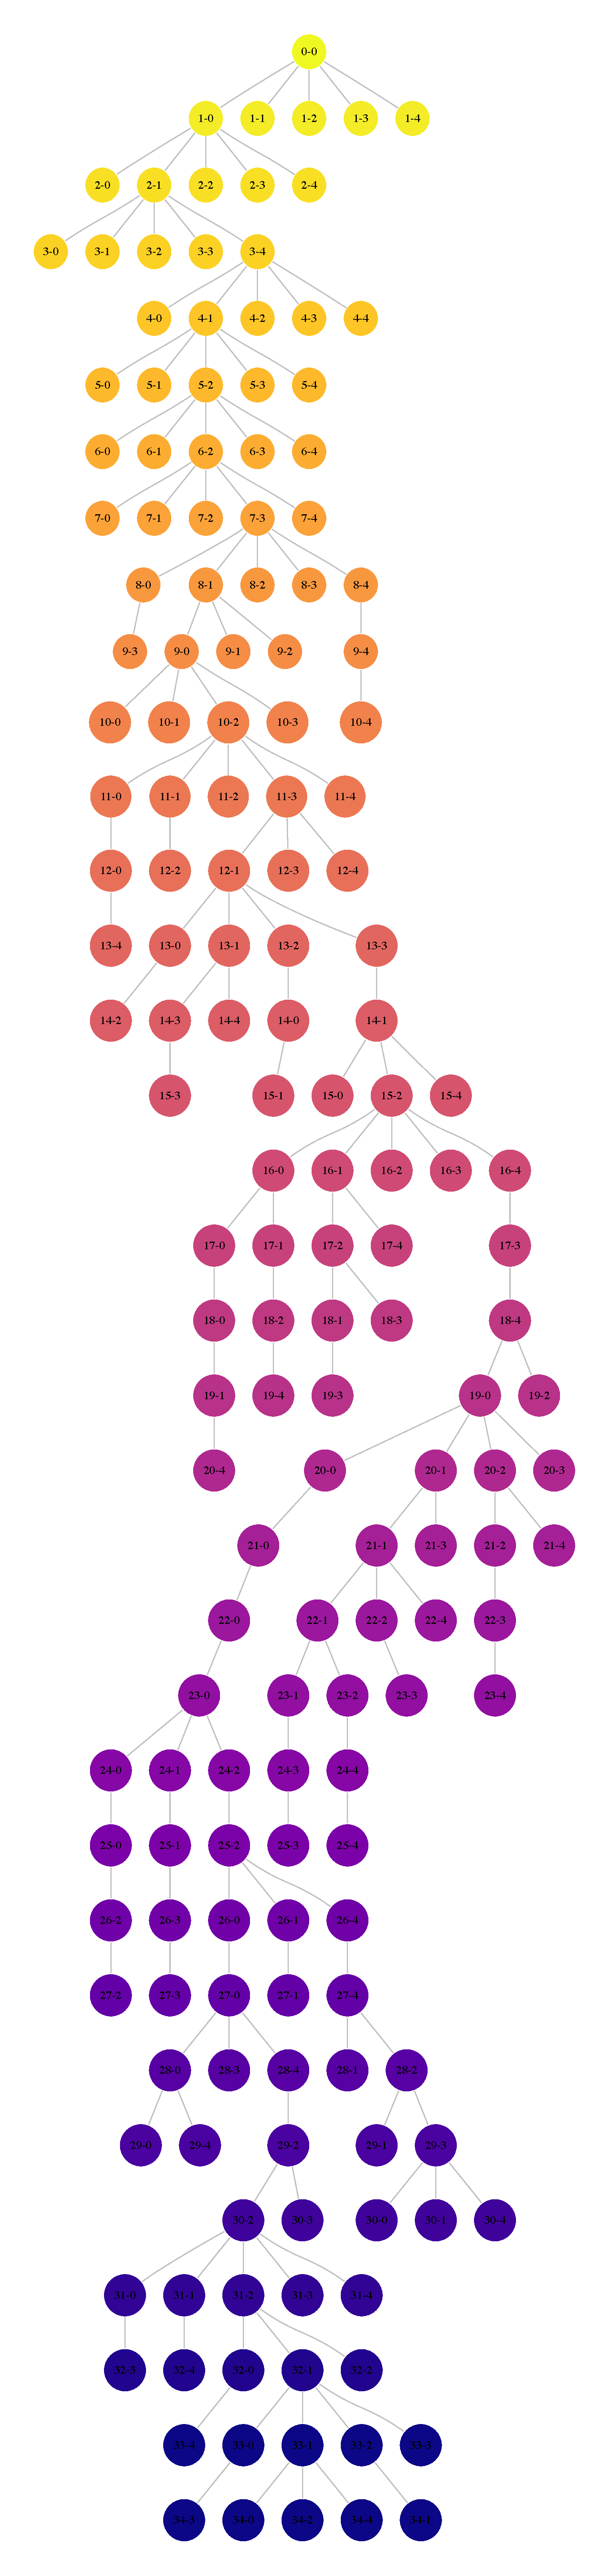
\includegraphics[scale=0.08]{Figures/tree_chi_pacs_best.pdf}
 \subcaption{PaCS}
 \end{minipage}
 \begin{minipage}{0.6\hsize}
 \centering
 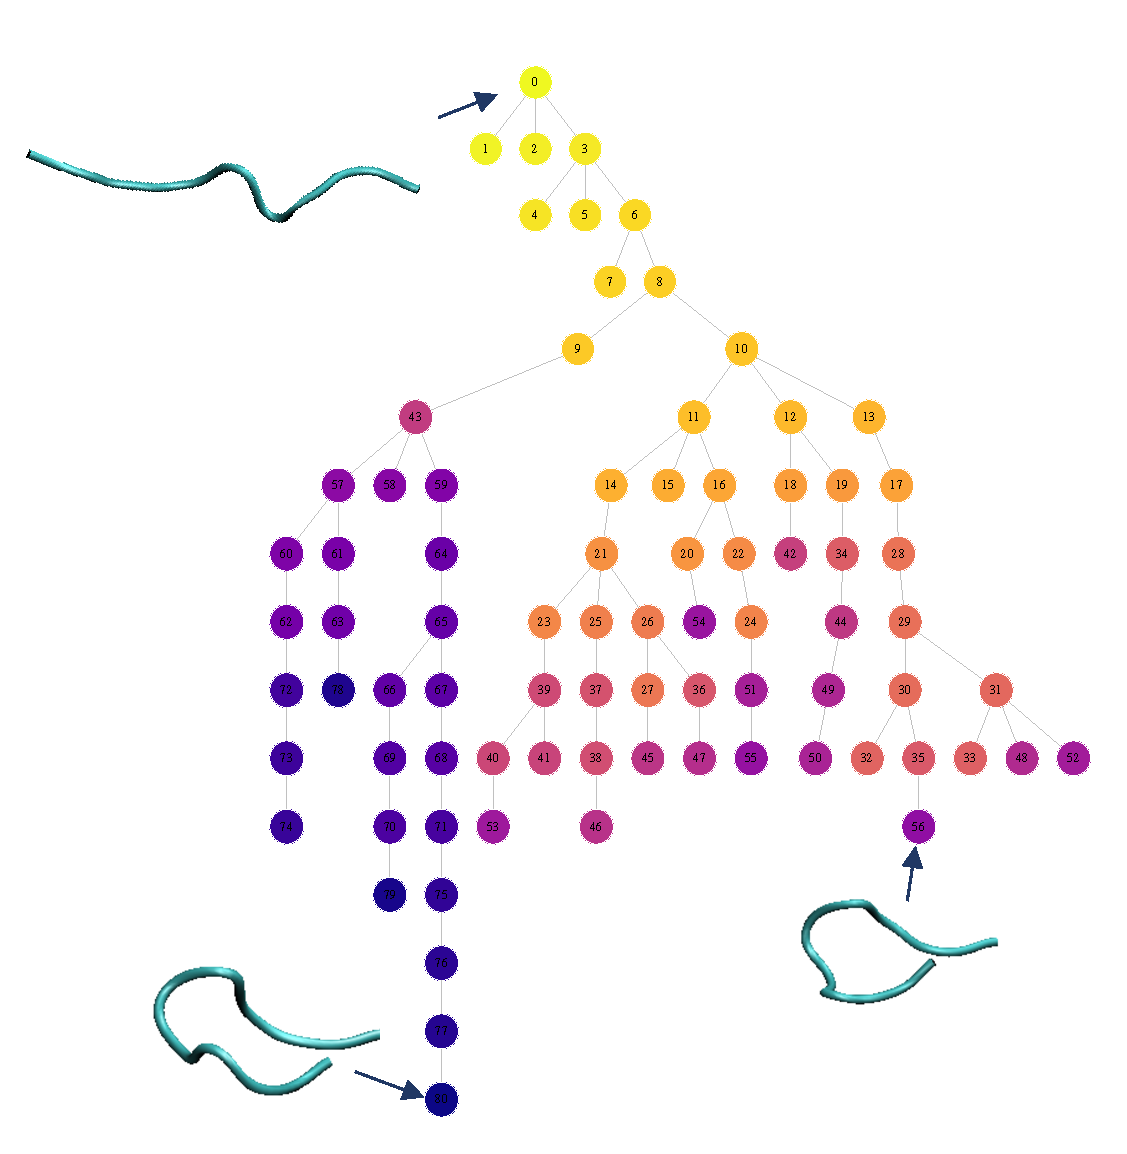
\includegraphics[scale=0.3]{Figures/tree_chi_pats.pdf}
 \subcaption{PaTS}
 \end{minipage}
\begin{minipage}{0.95\hsize}
\centering
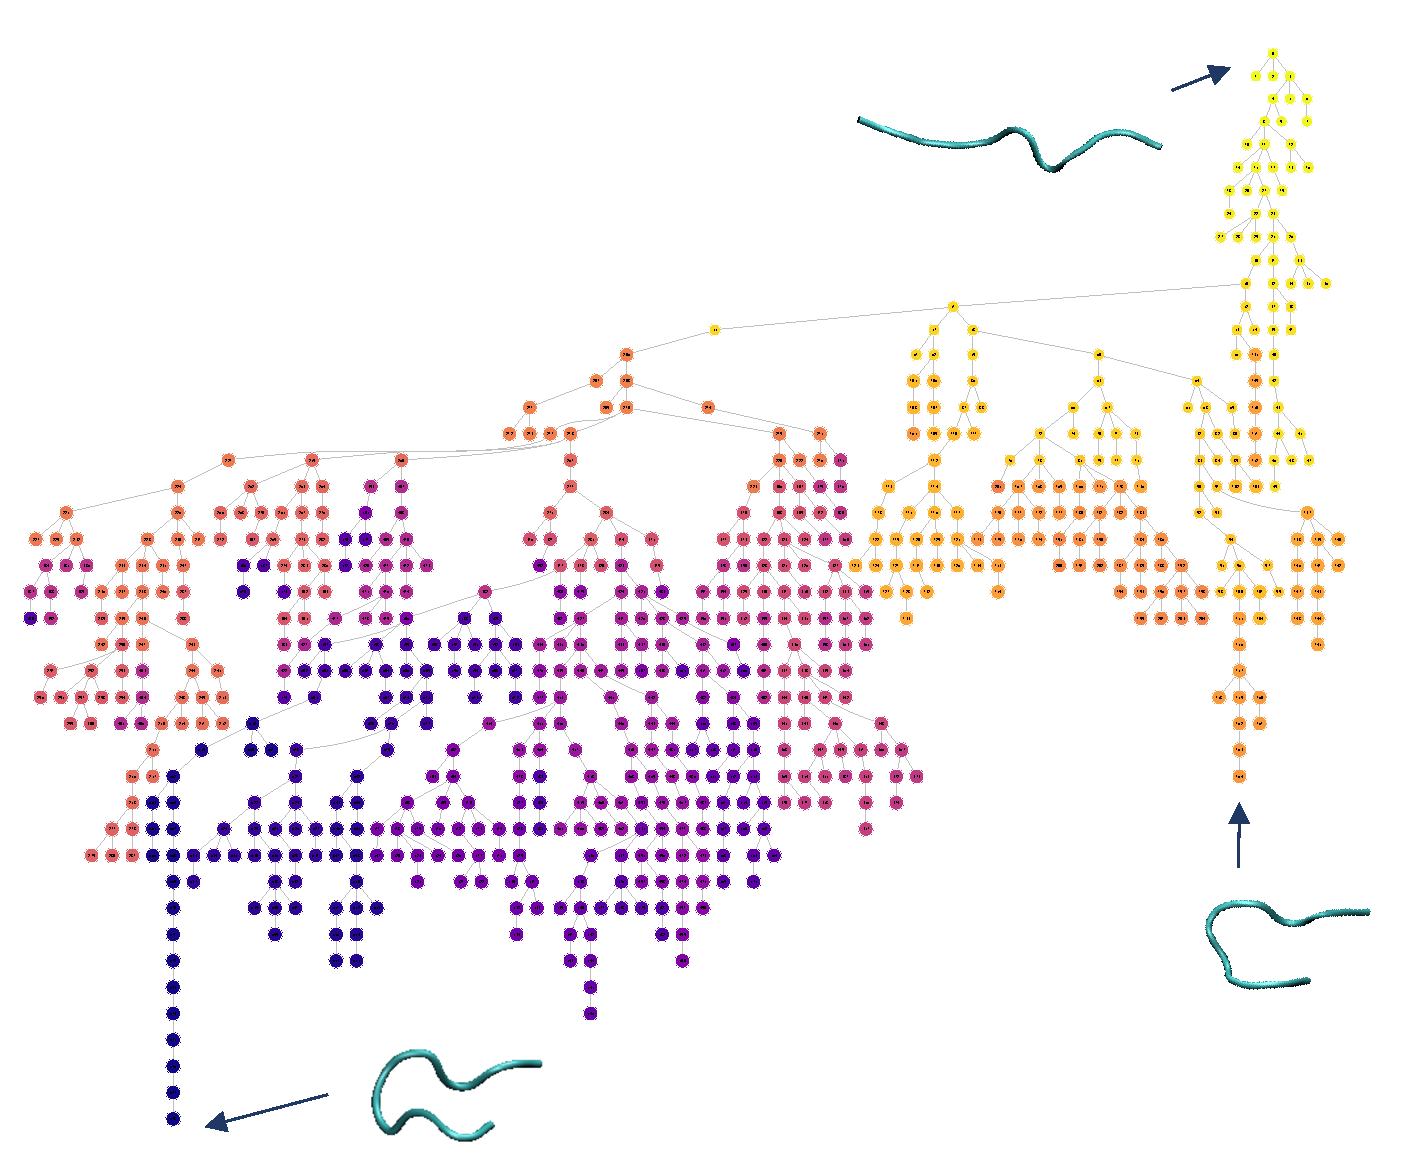
\includegraphics[scale=0.5]{Figures/tree_chi_pats_penal.pdf}
\subcaption{PaTS penalization}
\end{minipage}
\caption{Trees of Chignolin folding in each methods}
\label{fig:tree_chig}
\end{figure}

\begin{figure}[t]
\centering
 \begin{minipage}{1.0\hsize}
 \centering
 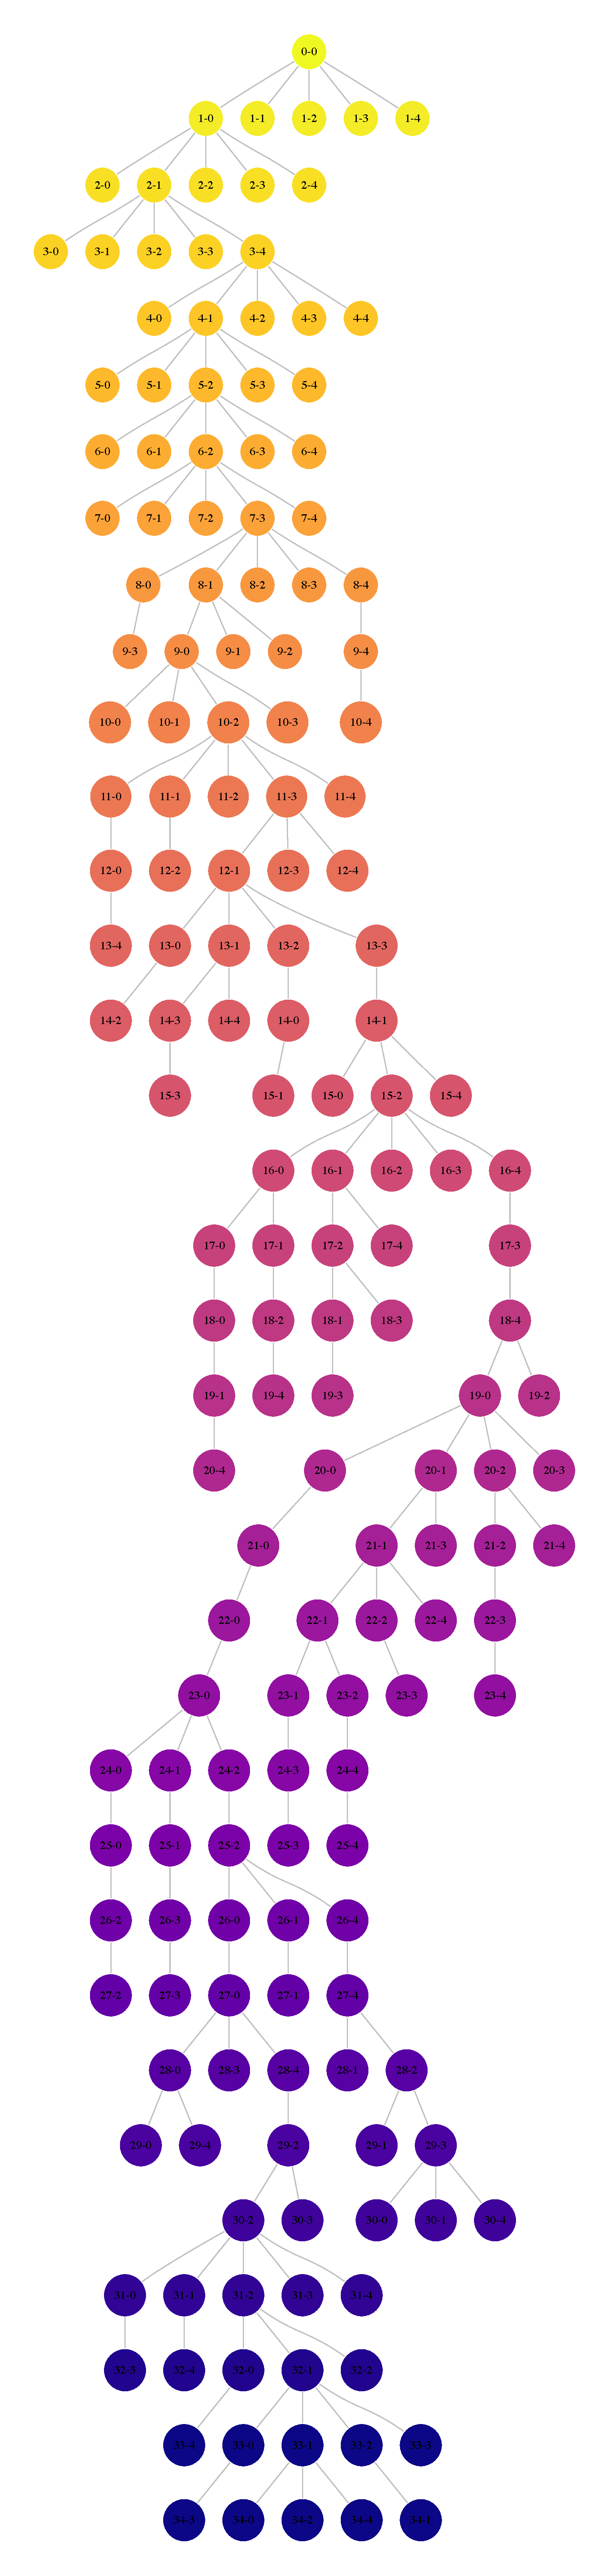
\includegraphics[scale=0.03, angle=90]{Figures/tree_chi_pacs_best.pdf}
 \subcaption{PaCS}
 \end{minipage}
 \begin{minipage}{1.0\hsize}
 \centering
 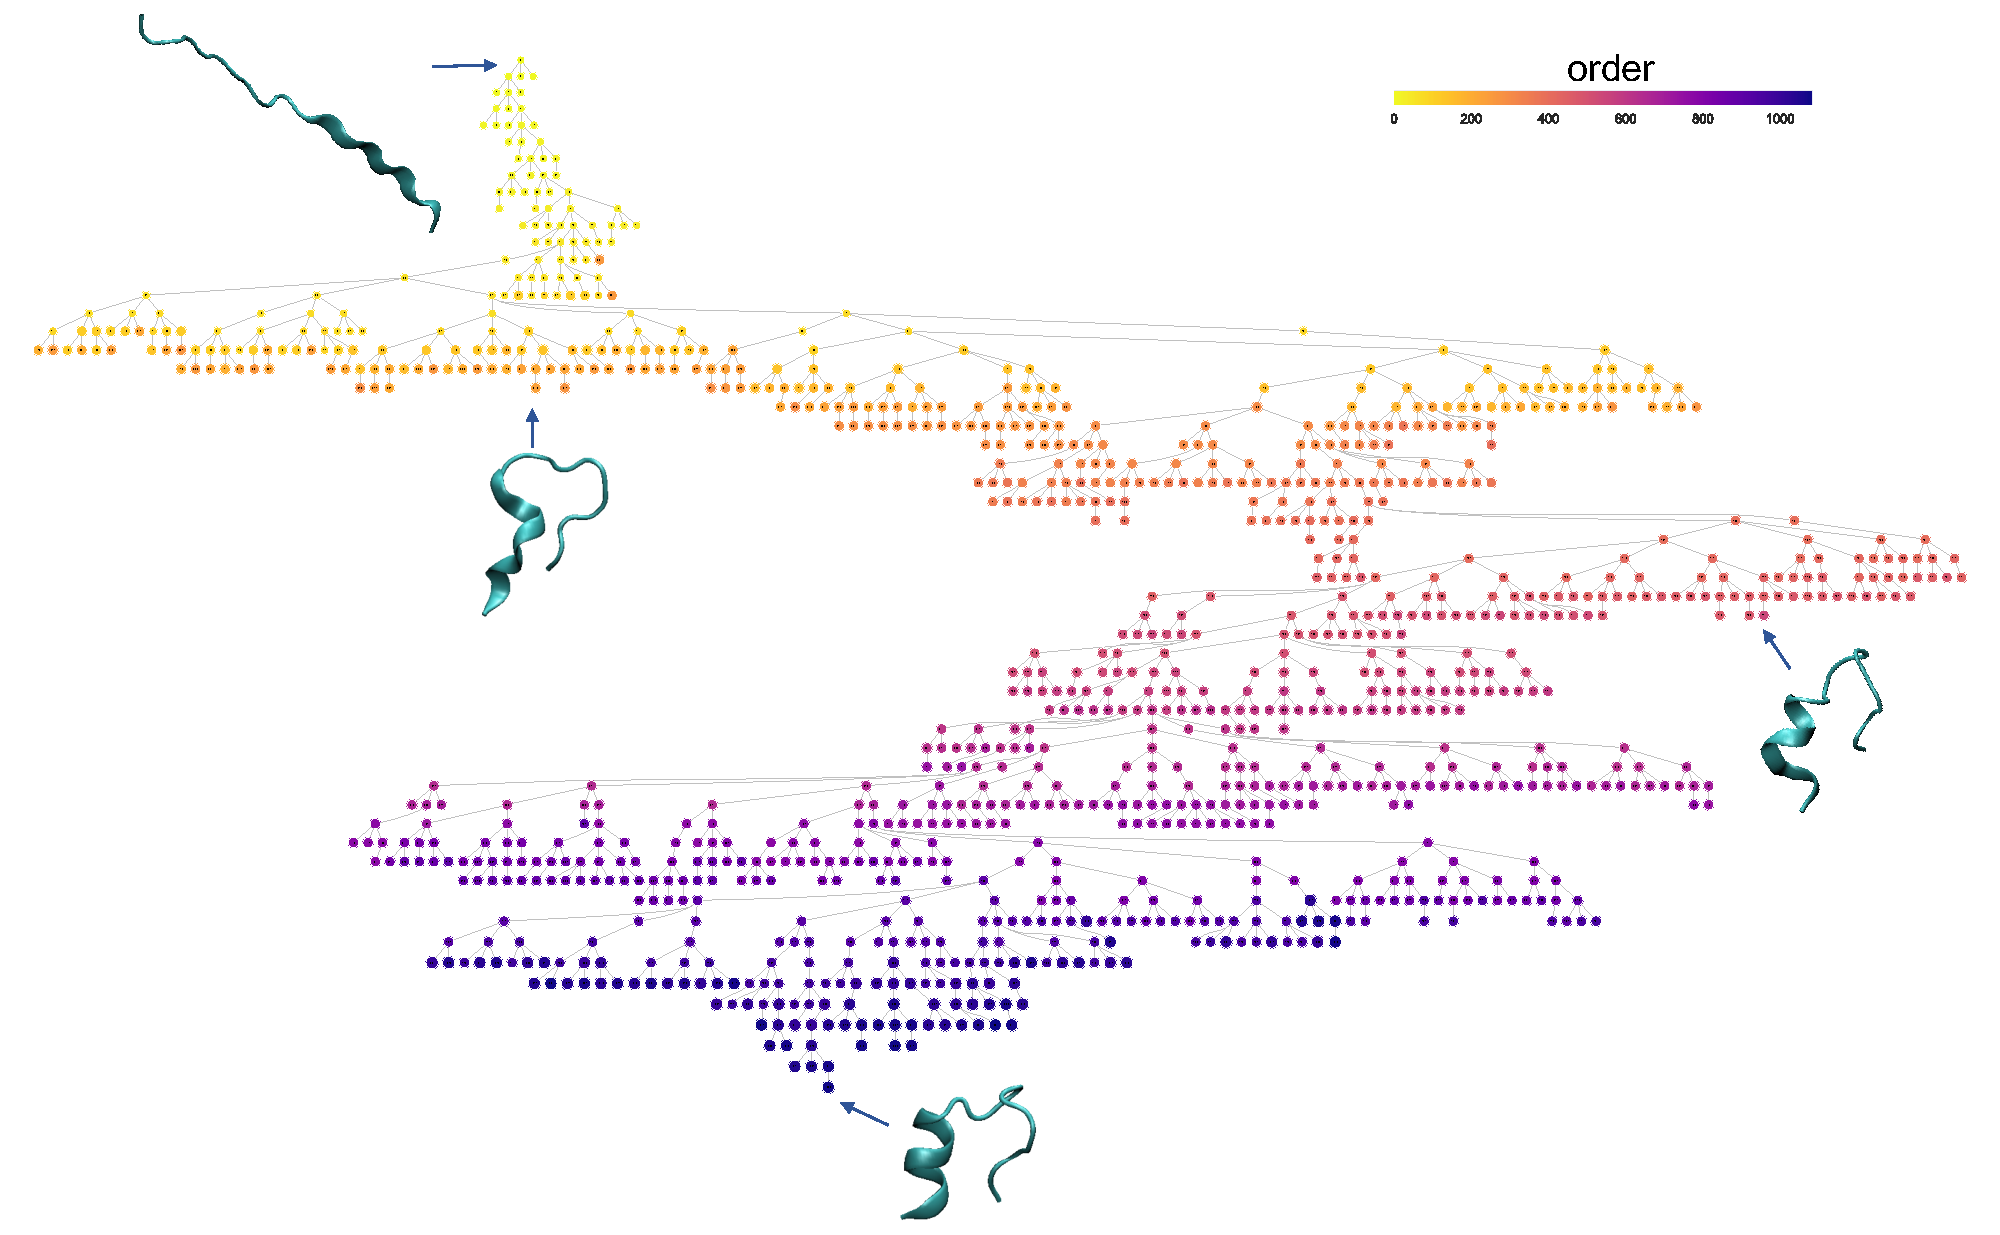
\includegraphics[scale=0.4]{Figures/tree_trp_pats_best.pdf}
 \subcaption{PaTS}
 \end{minipage}
\begin{minipage}{1.0\hsize}
\centering
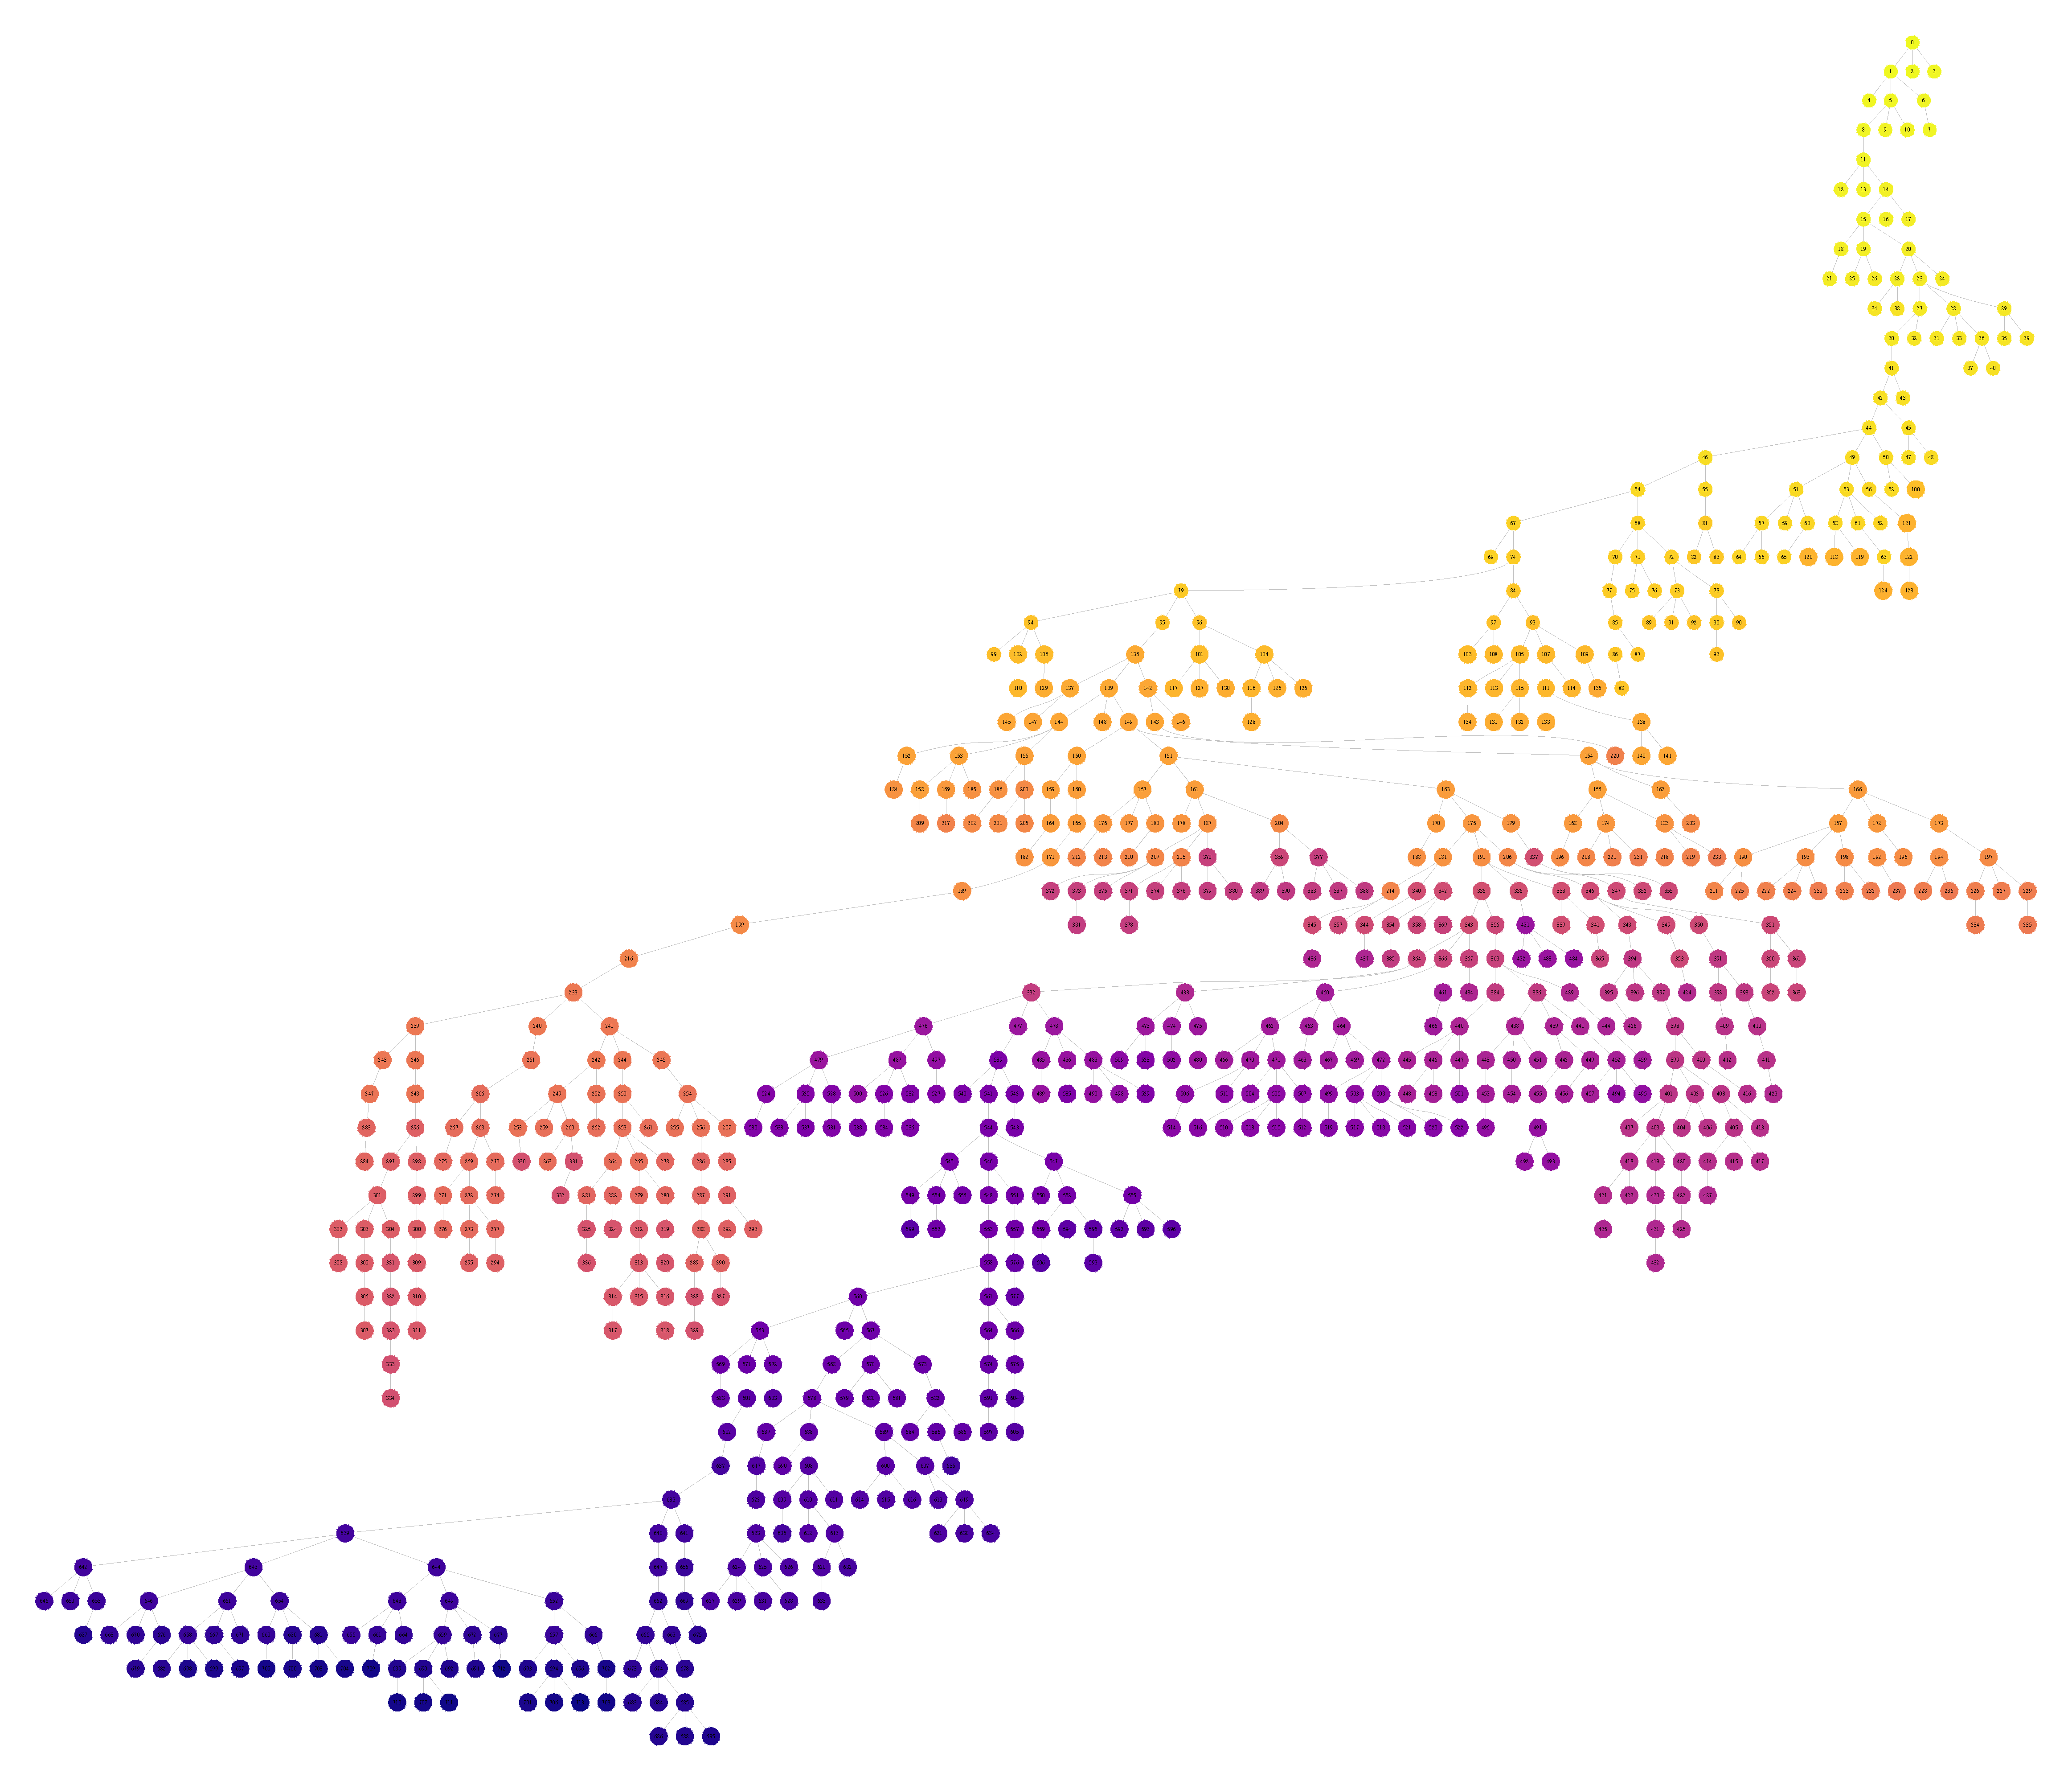
\includegraphics[scale=0.15]{Figures/tree_trp_pats_penal.pdf}
\subcaption{PaTS penalization}
\end{minipage}
\caption{Trees of Trp-cage folding in each methods}
\label{fig:tree_trp}
\end{figure}


